\documentclass[10pt, final]{article}

\usepackage{cite}
\usepackage{fullpage}
\usepackage{graphicx}
\usepackage{hyperref}
\usepackage{subcaption}
\usepackage{url}

% Line break with additional spacing. Default is .75 line-height extra spacing
% Extra space is put in to allow line breaks immediately after \item
\newcommand{\br}[1][.75]{\ \\[#1\baselineskip]}

\parindent 0pt

\begin{document}

\begin{center}
\LARGE{\textbf{Training a Pok\'{e}mon Puzzle League Champion}}\\
\Large{\textbf{CS 221 Project Proposal}}\\
\Large{Logan Short, Christopher Wong}
\end{center}

\section{Introduction}
Puzzle games have always served as ideal problems for the exploration and progression of artificial intelligence methodology. In this paper, we explore the development of an AI agent for the video based puzzle game, Pok\'{e}mon Puzzle League, released by Nintendo in September 2000 for the Nintendo 64 entertainment system.

\section{Task Definition}
Pok\'{e}mon Puzzle League is played on a grid-based board 6 tiles wide and 12 tiles tall. Each space in the board can be occupied by a block, which can be one of several types. Players control a freely moving cursor that encapsulates 2 horizontally adjacent grid squares. At any time, the player can choose to swap the positions of the two blocks currently selected by the cursor. If there ever exists a series of $3$ or more blocks of the same type in a line, these blocks are cleared from the board. New blocks will slowly appear from the bottom, causing the entire grid to continuously rise to the top. If the blocks reach the top, the player loses.\br
There are $1$-player and $2$-player modes for the game. In the $1$-player ``Endless'' mode, the human player plays for as long as possible, attempting to get the highest score before losing. In the $2$-player ``Versus'' mode (see Appendix, Figure~\ref{fig:screenshot}), clearing many blocks quickly causes garbage blocks to be sent to the opponent's board, with the goal being to outlast one's opponent. Our project aims to create an automated agent that is capable of playing Pok\'{e}mon Puzzle League at a high level. Since optimal game strategy is largely the same in both modes, we will attempt to maximize our score in ``Endless'' mode and beat the in-game CPU consistently in ``Versus'' mode. We note that the in-game CPU can play at various difficulties.

\section{Literature Review}
We reviewed various research papers relevant to our topic, and many of them were influential in our design and approach (see Section $4$). Here, we summarize two of the most significant pieces.

\subsection{\href{https://http://cns-classes.bu.edu/cn550/Readings/frey-slate-91.pdf}{Letter Recognition using Holland-Style Adaptive Classifiers} (Frey and Slate, 1991)}
In \cite{1}, Frey and Slate utilize an adaptive classifier to successfully recognize letters from images. The classifier implemented by the paper constructs $16$-dimensional feature vectors that can be used to represent images with features being selected to represent certain characteristics that different letters in the English alphabet might possess. A dataset consisting of character images from $20$ different fonts with slight alterations, such as scaling or rotation, was then used to train the classifier. Frey and Slate found that, by utilizing this approach, they were able to achieve high levels of accuracy for English letter prediction.

\subsection{\href{https://hal.inria.fr/inria-00418954/document}{Building Controllers for Tetris} (Thiery and Scherrer, 2009)}
In \cite{2}, Thiery and Scherrer provide an overview of the three most successful methods for automated playing of the video game Tetris. The first two, hand-written evaluation and general purpose optimization both attempt to optimize weights for features that represent the quality of a move. These two methods are noted to have achieved the most success in Tetris gameplay. Reinforcement learning attempts to learn a policy for achieving an optimal expected future score. Thiery and Scherrer point out that Tetris might be too complicated of a game for state-of-the-art reinforcement learning approaches; thus these methods have not been as successful.

\section{Approach}
\subsection{Board Recognition}
Since we do not have access to the internal data of the game, we can rely only on what is being displayed on screen. Thus, given a screenshot of the game, our first challenge is to be able to detect the board's grid state with $100\%$ accuracy. Since this step is critical to determining the feasibility of our project, we have already implemented a good portion of this infrastructure. We first built an interface to the game that allows us to send movements and capture screenshots multiple times per second.\br
Next, from a screenshot, we extract and classify the grid squares from the agent's board (see Appendix, Figure~\ref{fig:extract}). To do so, we used OpenCV to isolate and divide the board. We then used a logistic regression classifier to determine the type of each block. In our first implementation, our features for each block image were simply the RGB values of each pixel. However, one remaining challenge will be differentiating an active grid block from an empty background. Inspired by \cite{1}, we are hoping that to use more effective features -- for example, considering the standard deviation in color -- to solve this problem. Another challenge is that the grid varies in position, since blocks slowly rise from the bottom. To solve this, we consider the block-sized image at each possible vertical position of the lower left block. Using our classifier, we calculate the likelihood that each image is an actual block, and we pick the position that yields the highest probability.

\subsection{Best Move Calculation}
Now, given any board, our agent must calculate the best move possible. Based on the results of \cite{2}, Pok\'{e}mon Puzzle League is likely too complex of a game for reinforcement learning approaches. Consequently, our current approach revolves around a heuristic-based identification of ideal board states and a move-by-move progression towards said game states using A* search. Gameplay in both ``Endless'' and ``Versus'' modes favors clearing a large number of pieces in a small amount of time, so the potential to quickly clear pieces plays a central role in our board evaluation. At a high level, reinforcement learning methods such as MDP seem well tailored for puzzle games such as Pok\'{e}mon Puzzle League. Therefore, we have not yet ruled out reinforcement learning as a method for best move calculation. We will continue to explore approaches that maximize the potential of reinforcement learning, perhaps in combination with our A* search.\br
We note that optimization will be a critical part in our development process. To be an effective player, our agent needs to make around $4$ to $8$ moves per second. This means, on average, we will need to able to take a screenshot, parse the game state, calculate the best move, and send the move to the game every $0.2$ seconds.

\subsection{Evaluation}
As mentioned in Section $2$, we can evaluate our agent's performance in both ``Endless'' and ``Versus'' mode. In particular, with respect to the game's scoring system, we want to maximize score in ``Endless'' mode, and in ``Versus'' mode, we want to beat the in-game CPU player consistently. Using our already built-out infrastructure described in Section $4.1$, we implemented a baseline AI that makes $5$ random moves per second. Since the board position itself changes in each mode, we have only evaluated our baseline in ``Versus'' mode so far. We plan to gather baseline scores in ``Endless'' mode very soon. For an oracle, we played the game ourselves, since we were the best game players that we could find, human or machine. Below are our results. Since the game is complicated, we can see the baseline AI does not do well at all.
\begin{center}\begin{tabular}{l||c|c|c|c|c}
Opponent CPU Level & Easy & Medium & Hard & Very Hard & Super Hard \\ \hline \hline
Baseline Wins ($10$ games) & 2 & 1 & 0 & 0 & 0 \\ \hline
Oracle Wins ($10$ games) & 10 & 10 & 9 & 7 & 1
\end{tabular}\end{center}
\newpage

\section{Appendix}
\begin{figure}[h!]\begin{center}
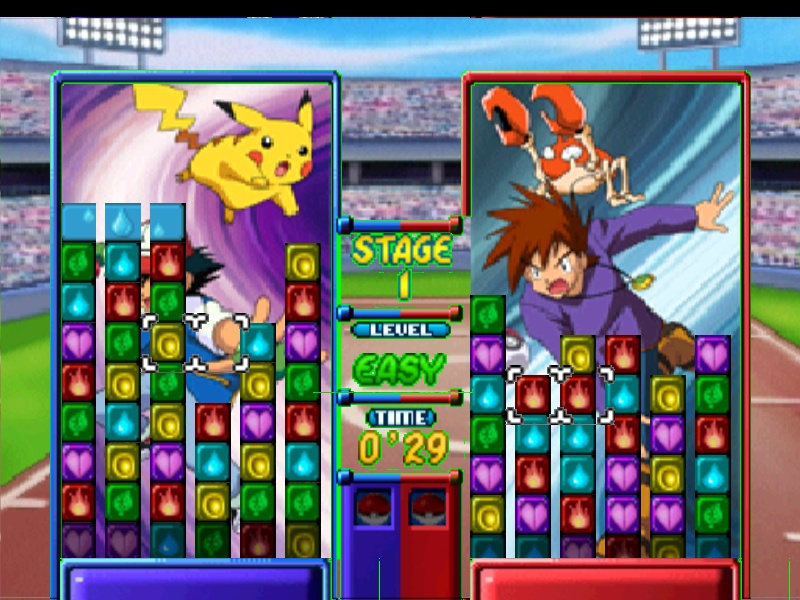
\includegraphics[width=3.4in]{game.jpg}
\caption{Example game screen in $2$-player mode. The human player or agent is on the left.}
\label{fig:screenshot}
\end{center}\end{figure}
\begin{figure}[h!]\begin{center}
\begin{subfigure}[h]{1.6in}
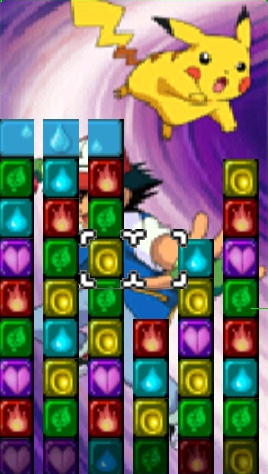
\includegraphics[width=1.6in]{board.jpg}
\caption*{Isolate the agent's board.}
\end{subfigure}
~$\mathbf{\Longrightarrow}$~
\begin{subfigure}[h]{1.6in}
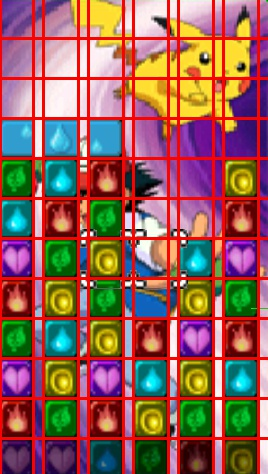
\includegraphics[width=1.6in]{grid.jpg}
\caption*{Divide board into a grid.}
\end{subfigure}
~$\mathbf{\Longrightarrow}$~
\begin{subfigure}[h]{1.2in}
  \begin{subfigure}[h]{.5in}
  
\includegraphics[]{square0.jpg}
  \caption*{$(0,0)$}
  \end{subfigure}
  ~
  \begin{subfigure}[h]{.5in}
  
\includegraphics[]{square1.jpg}
  \caption*{$(0,1)$}
  \end{subfigure}
  \caption*{Extract squares.}
\end{subfigure}
\caption{Process of parsing the grid game state from the game screen.}
\label{fig:extract}
\end{center}\end{figure}

\begin{thebibliography}{1}
\bibitem{1} P. Frey, D. Slate. Letter Recognition using Holland-Style Adaptive Classifiers. ML, 1991.
\bibitem{2} C. Thiery, B. Scherrer. Building Controllers for Tetris. ICGA, 2009.
\end{thebibliography}

\end{document}